\section{Literature review method}~\label{rw-tactics-and-topics-for-this-chapter}

Where others have done similar work they've done so in other ways \emph{e.g.} \Gls{msr} and/or \Glspl{slr} rather than focusing on the development teams. While their work is tremendously interesting it does not take the perspective of app developers. Further there is limited prior research that focuses on the use of mobile analytics or effects of analytics on the quality of the mobile apps produced and their related artefacts. 


\begin{figure*}
    \centering
    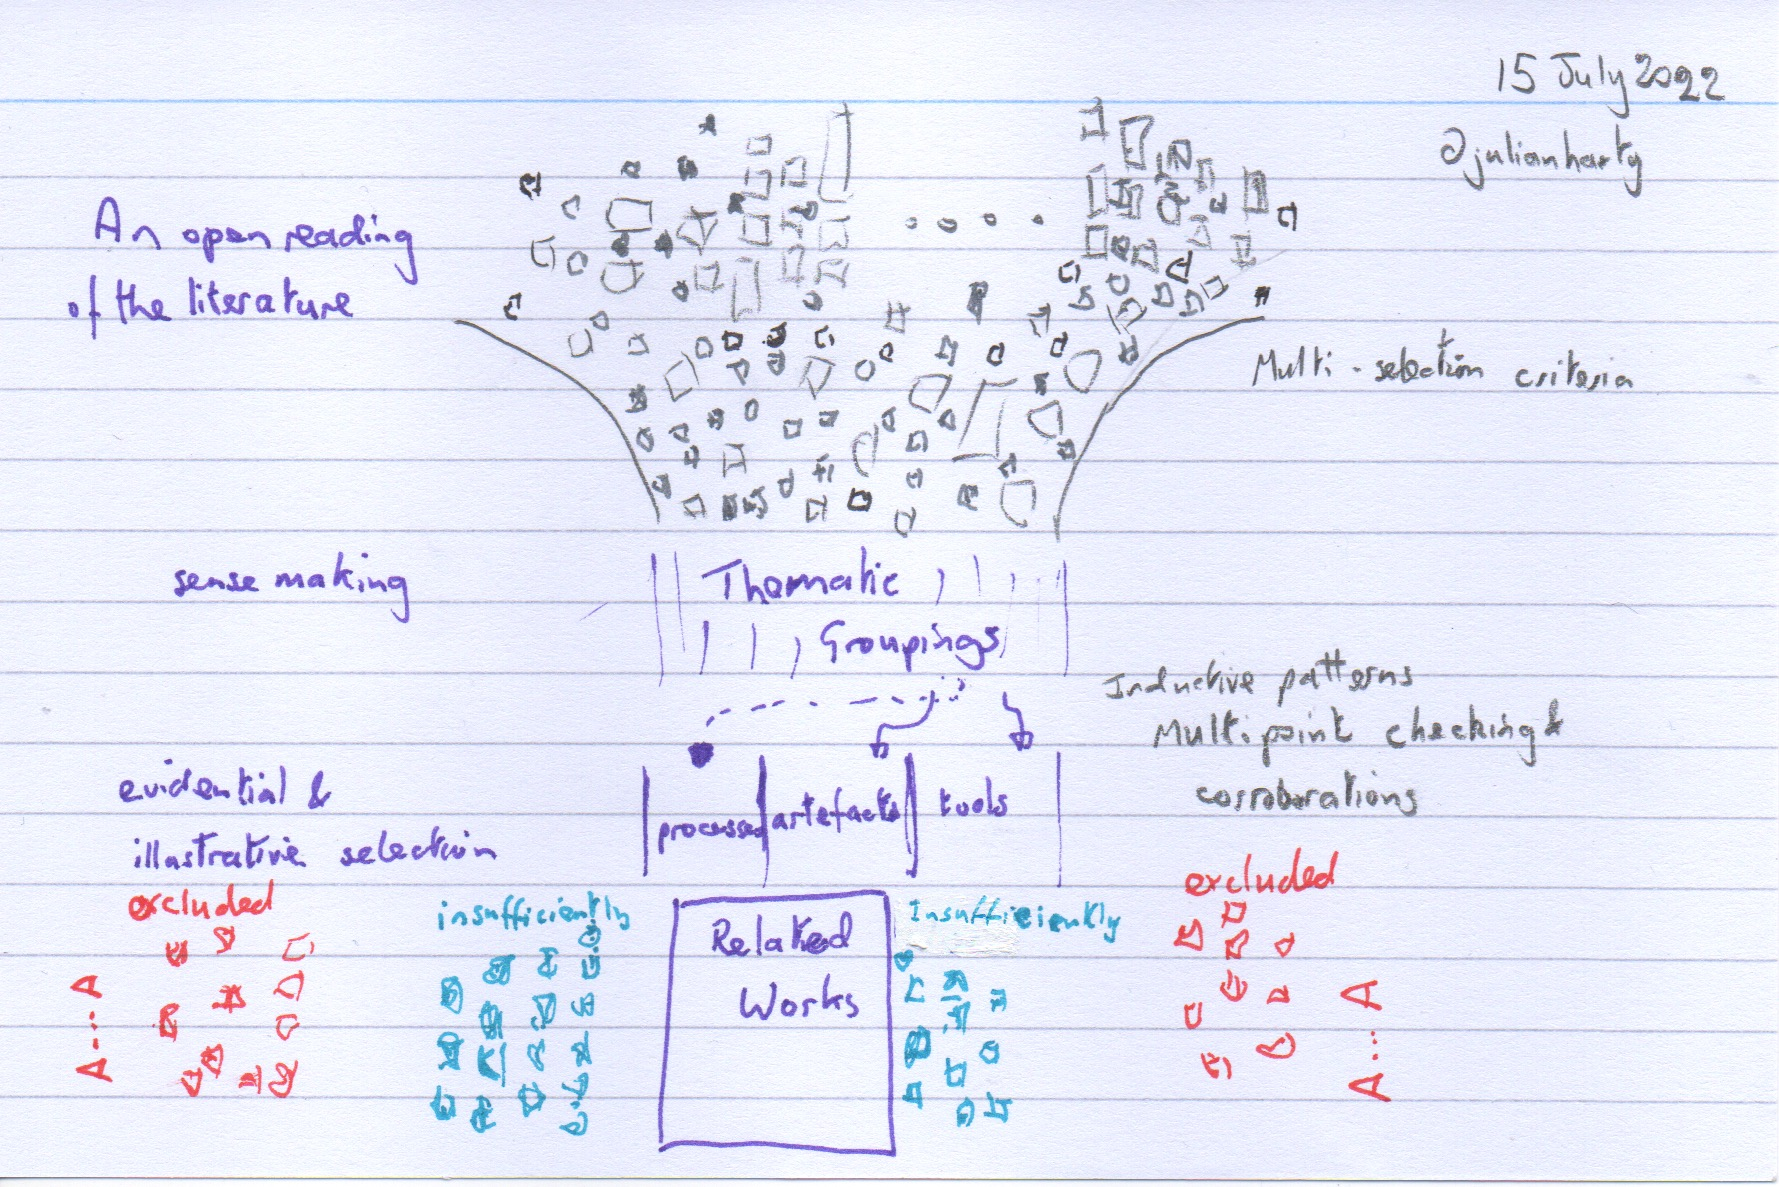
\includegraphics[width=\textwidth]{images/rough-sketches/literature-review-overview.jpeg}
    \caption{Overview of the literature review process and outcomes}
    \label{fig:literature-review-overview}
\end{figure*}

Figure \ref{fig:literature-review-overview} illustrates my approach to researching prior work in the use of mobile analytics by app developers. 
%
The initial trawl for prior work was based on searching for scholarly articles and accounts of software development practices that included different combinations covering the concepts of: ``software quality'', ``reliability'', ``stability'', ``mobile applications'', "software development", "software release practices", ``software analytics'', ``crashes'', ``crash analytics'', ``ANR'', and ``mobile analytics''. These were also combined with additional search terms including: "app store", ``Android'', and ``iOS'' to seek publications that were more likely to be germane to the research questions.  

These search results led to various additional searches, including keyword, tags, and related items, that were incorporated into the searches. Many of these searches were inductive, to seek information, patterns, nuggets of research interest, and so on. Other searches were stimulated by events and findings in the case studies.

Initial sources included Google Scholar to find the more research oriented materials and Google Search particularly for grey materials. Specialist search tools were used where sites provided them, for instance on stack exchange sites such as StackOverflow, GitHub.com, acm.org, ieee.org, and medium.com their respective search engines were used frequently. Where practical copies of material has been preserved privately and backed up using at least one commercial, paid-for, cloud file storage service~\sidenote{\emph{i.e.} Dropbox.} for safekeeping and to preserve evidence.

Multi-selection criteria were used to select material that appears of interest, relevant, and plausible. Generally bibliographic entries were obtained and these where checked for accuracy and completeness. Grey material seldom has a bibliographic entry, these were created by hand, and preserved. Snowball sampling helped increase the breadth of the search results. Termination of searches was based on reaching a point of diminishing returns in terms of new information. Selection was based on relevance to the research and to the case studies as elaborated below.

The results of the searches were filtered, for example, to remove papers that were not relevant to software development practice and those that focused on research tools that were not in use by practitioners. This was based on reading the title, abstract, and conclusions of the paper in the first instance, and exploring the findings in greater depth when needed. Similarly research into mobile apps and app stores that predated the introduction of mobile analytics was frequently filtered-out as \emph{de-facto} it did not include these aspects.

In reading the literature various \textit{false friends} emerged, papers that first appear relevant because of their titles and/or abstracts but turn out to be on very different topics. 
Knowing about the concept of false friends and having pragmatic strategies to deal with them is important to avoid misunderstandings or misleading application of their work, 
based on \sidecite[][p. 1833]{chamizodominguez2002_false_friends_their_origins_and_semantics_in_some_languages}. 

Through a process of sense-making\index{Sense-making method}, cross-checking, and corroborations, various thematic groupings emerged together with potential relationships between the thematic groups. Based on this analysis three clearly distinct and vital aspects emerged in the related work - the development practices used by mobile app developers, the artefacts they create and maintain, and the mobile analytics tools the developers use. These were further refined into six perspectives that considered the current \emph{what is}, and \emph{what might be} in terms of making improvements, for each aspect. 

